% 
% Annual Cognitive Science Conference
% Sample LaTeX Paper -- Proceedings Format
% 

% Original : Ashwin Ram (ashwin@cc.gatech.edu)       04/01/1994
% Modified : Johanna Moore (jmoore@cs.pitt.edu)      03/17/1995
% Modified : David Noelle (noelle@ucsd.edu)          03/15/1996
% Modified : Pat Langley (langley@cs.stanford.edu)   01/26/1997
% Latex2e corrections by Ramin Charles Nakisa        01/28/1997 
% Modified : Tina Eliassi-Rad (eliassi@cs.wisc.edu)  01/31/1998
% Modified : Trisha Yannuzzi (trisha@ircs.upenn.edu) 12/28/1999 (in process)
% Modified : Mary Ellen Foster (M.E.Foster@ed.ac.uk) 12/11/2000
% Modified : Ken Forbus                              01/23/2004
% Modified : Eli M. Silk (esilk@pitt.edu)            05/24/2005
% Modified: Niels Taatgen (taatgen@cmu.edu) 10/24/2006

%% Change ``a4paper'' in the following line to ``letterpaper'' if you are
%% producing a letter-format document.

\documentclass[10pt,letterpaper]{article}

\usepackage{cogsci}
\usepackage{pslatex}
\usepackage{apacite}
\usepackage{graphicx}


\title{Basal ganglia-inspired functional constrains improve the robustness of $Q$-value estimates in model-free reinforcement learning}
 
\author{{\large \bf Patrick J. Rice (pjrice@uw.edu)} \\
  Department of Psychology, University of Washington \\
  Seattle, WA 98195 USA
  \AND {\large \bf Andrea Stocco (stocco@uw.edu)} \\
  Department of Psychology, University of Washington \\
  Seattle, WA 98195 USA}


\begin{document}

\maketitle


\begin{abstract}
The abstract should be one paragraph, indented 1/8~inch on both sides,
in 9~point font with single spacing. The heading {\bf Abstract} should
be 10~point, bold, centered, with one line space below it. This
one-paragraph abstract section is required only for standard spoken
papers and standard posters (i.e., those presentations that will be
represented by six page papers in the Proceedings).

\textbf{Keywords:} 
Add your choice of indexing terms or keywords; kindly use a semi-colon; between each term.
\end{abstract}


\section{General Formatting Instructions}


Model-free reinforcement learning (RL) is a powerful approach for obtaining an optimal long-term action policy 
in the absence of transition probability and reinforcement functions. 
In other words, a model-free RL agent must interact with an unknown environment (i.e. sample the environment 
repeatedly through action) in order to construct an optimal control policy, based on the pattern of 
reward received by interaction with the environment. This policy is oriented such that 
the agent’s actions consider both immediate and future reward, optimized to maximize some value over time.
The key idea that enables an agent to determine an optimal policy within an unknown environment is that
of temporal-difference (TD) learning (Sutton and Barto, 1988). Under TD learning, an agent 
estimates the values of states on-line (during exploration of the environment) through the updating
of a state-dependent value function. This value function estimates the value of the current state, 
and is updated once the agent performs an action in order to transition to a different state, which 
results in the receipt of some reward. Upon reward receipt, the value function is updated by the weighted 
sum of the estimated value of the reward of all future steps (beginning from the current state, modulated by 
some learning rate alpha. These estimated state values can then be directly used to implement a policy to 
select actions on the basis of those that lead to states that are estimated to return the greatest value over time.

% THE MODEL AS WRITTEN IS ACTUALLY A SARSA MODEL – CHANGE THE FOLLOWING 
% PARAGRAPH? 
% [AS] Nope, since it does not matter how the model is written---In PSS, the second action does not matter, so Q(a_t2) can be considered zero.

The ideas behind TD methods have since been expanded, including a proposal by Watson (1989) that defined a TD control algorithm now known as Q-learning. Q-learning is an off-policy method that allows the agent to choose to take non-optimal actions while still estimating an optimal value function. In comparison to the TD method described above, Q-learning carries two essential differences: 1. the method considers the value of state-action (SA) pairs, rather than the value of states alone (however, the two formalisms are equivalent (Sutton and Barto, 1998)); and 2. for each time-step, the learned action-value function is updated (in part) by the estimated value of the best action available, rather than the actual action taken. By updating based on the best action available while allowing the agent to make inferior choices, this procedure increases the rate of learning in the face of a suboptimal action selection process.

Both TD learning and Q-learning have been shown to converge to the optimal value function with probability 1 (CITE THIS). 

% This is where the juice happens.

However, in some circumstances, these model-free RL methods 
produce bizarre suboptimal results. As defined, these methods emphasize learning of rewarding actions--updating the value of a state/action
pair increases the likelihood that the agent will choose the same action in the same state again. 

As a result, even though it converges to an optimal value function, an agent still does not have complete knowledge of its environment---namely, it does not know much (if anything) about those actions that were discarded early as suboptimal. 

Note that this is not an issue while the agent has full access to its actions, but what if learned "good" (i.e. optimal) actions pairs become suddenly unavailable? In this case, the agent cannot take the actions it usually would by following its policy and value function, and as a consequence, cannot act optimally within the "new" environment. In essence, the agent has no knowledge of how to navigate bad options--how to choose the "least bad", when forced to.

\subsection{The PSS Task}

\begin{figure*}[ht]
	\begin{center}
		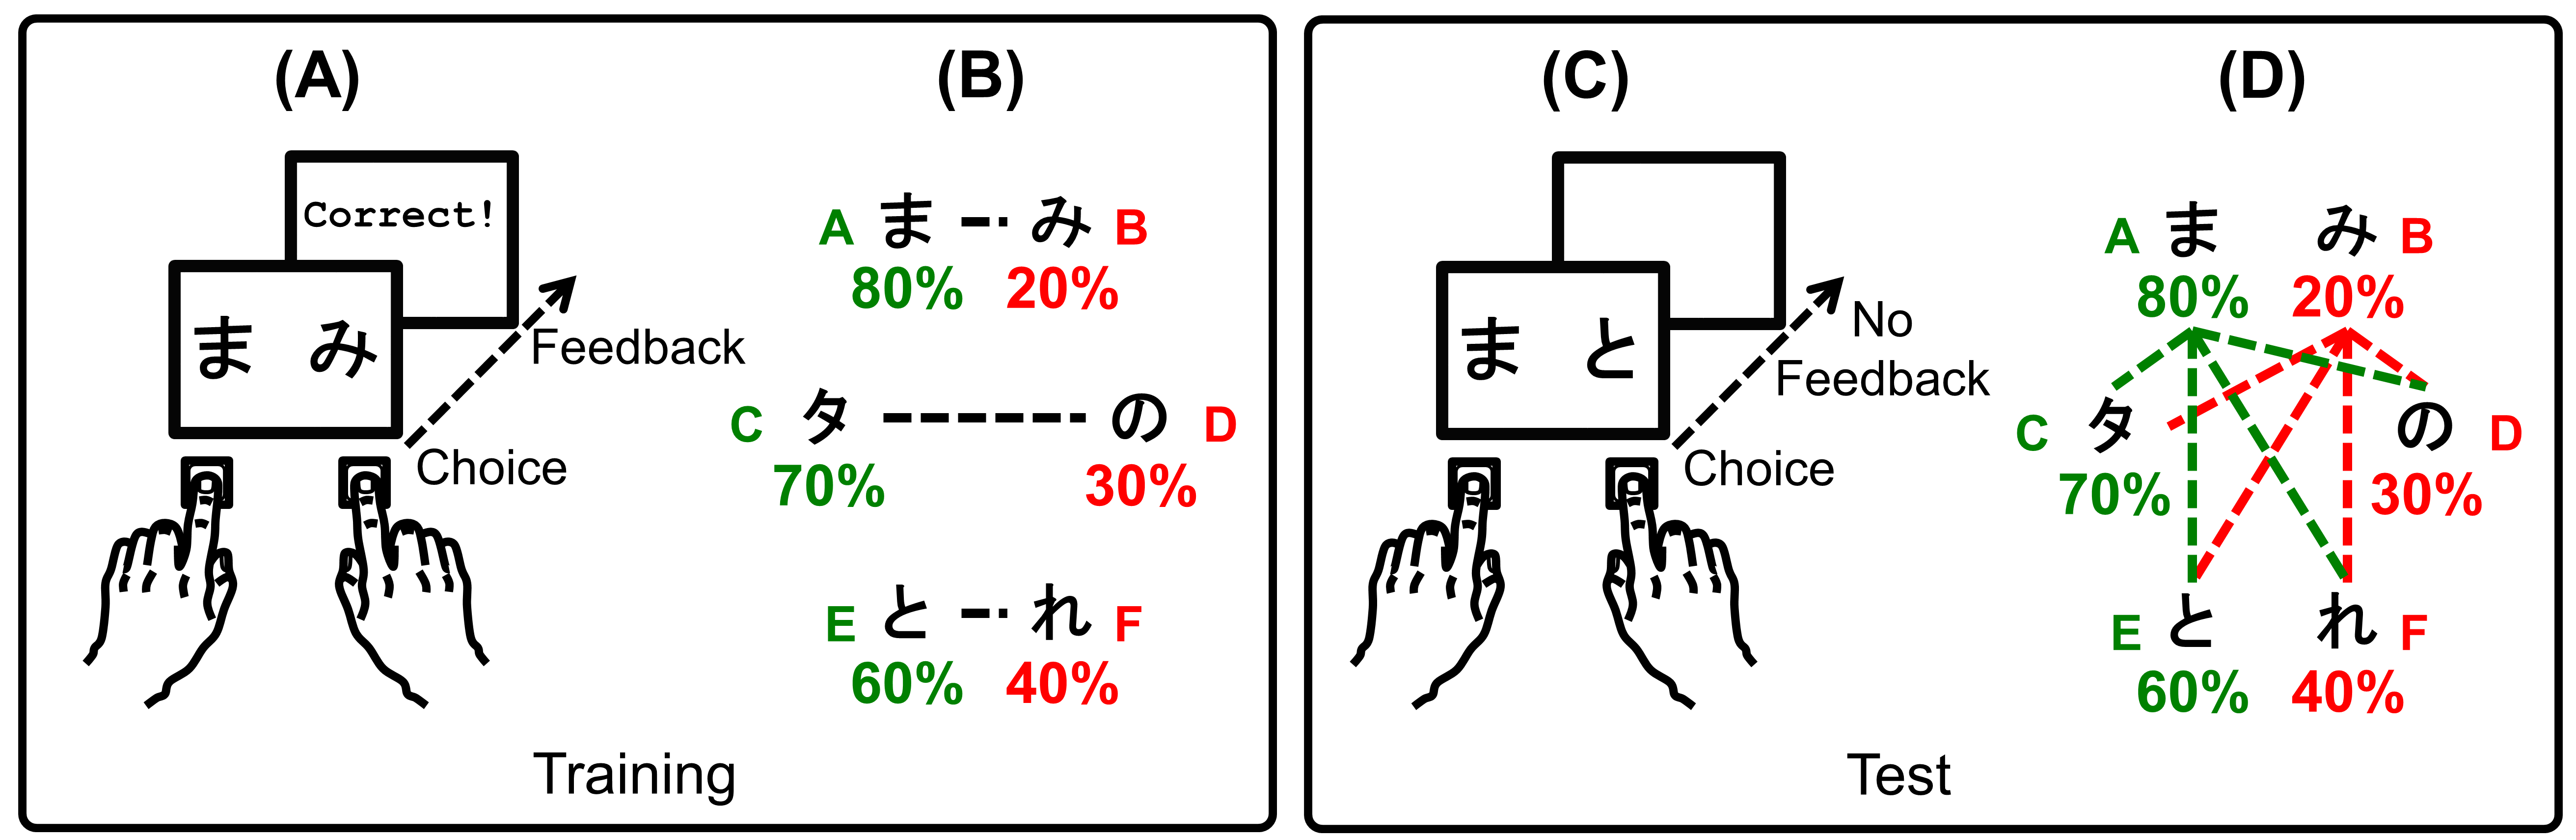
\includegraphics[width=\textwidth]{pss.png}
	\end{center}
	\caption{The PSS task} 
	\label{pss}
\end{figure*}

A situation in which this circumstance arises is when modeling a classical psychology task paradigm, the Probabilistic Stimulus Selection (PSS) task. The PSS task is a repetitive, two-alternative forced-choice task made up of two consecutive phases--a training phase in which a participant repeatedly makes choices between fixed pairs of stimuli, and a test phase where the participant is presented with new combinations of options. Across both phases, there are six possible stimuli, implemented as symbols that are difficult to describe (in order to make memorization of each stimulus’ history of success more difficult). Each stimulus carries an intrinsic probability of success, ranging linearly from 20\% to 80\%.

During the training phase, the stimuli are presented a fixed pairs, for a total of three sets (as in Figure \ref{pss}), and participants receive feedback regarding the outcome of their decision directly after making a selection. Participants are instructed to attempt to maximize their success by choosing what they believe to be the "correct" option on each trial. Once a participant’s performance reaches a predefined criterion (or they have completed a maximum of six training blocks), the test phase begins. During the test phase, participants are shown all possible combinations of the six stimuli(fifteen total, four times each, for a total of 60 trials), and do not receive feedback upon selection. From the test phase, two different measures are calculated: the participant’s Choose accuracy, (the probability of choosing the higher valued alternative (80, 70, or 60 – hereafter referred to as A, C, and E, respectively) of any given fixed set from the training session, when it is paired with any other alternative), and the participant’s Avoid accuracy (the probability of choosing the lower valued alternative (20, 30, 40 – hereafter referred to as B, D, and F, respectively) of any given fixed set from the training session, when it is paired with any other alternative). These measures can generally be interpreted to be the participant’s tendencies to pursue reward and avoid punishment, respectively.

%BRIEF PARAGRAPH ON HOW HUMANS DO AT THE PSS TASK? WOULD BE NICE TO %COMPARE MODEL RESULTS TO 
% We have millions of data.

When the participant in the PSS task is modeled as a Q-learning agent that employs either an epsilon-greedy (in which the agent selects the optimal action with probability $P = 1 - \epsilon$, and selects an action at random with probability $P = \epsilon$) or a policy based on Gibb’s function 

	EQN HERE
	
(under which the probability of the agent choosing a given action increases proportionally with the action’s value Q(s,a), normalized by a constant T, defined as the temperature of the system), some alarming results are observed. In both cases, the model learns the value of of the desirable options (A, C, or E) well, reflected as an increasing Choose accuracy as either epsilon or T decreases (Figure 1A,B). This is the expected behavior of the model – as exploration begins to suggest relatively “better” options, the model quickly switches to exploiting these options, learning their values well in the process.

However, when the Avoid accuracy of the model is inspected, it becomes clear that the model has learned the value of some, but not all, options well. In both cases, as either epsilon or T begins decreasing, the Avoid accuracy of the model does begin increasing, as the Choose accuracy did (these increases in Avoid accuracy are commensurate with the increases in Choose accuracy). However, at A CERTAIN POINT ON THE EPSILON/T AXIS, the model’s Avoid accuracy actually begins decreasing (Figure 1A,B). This indicates that for lower values of epsilon/T, the model does not sufficiently explore the “bad” options (B, D, and F) during the training phase, and as a consequence, does not value them appropriately. For higher values of epsilon/T, the model does explore both bad and good options approximately equally – however, it does not value neither good nor bad options appropriately. Additionally, the maximum Avoid accuracy achieved at the point of inflection (approximately 70\%) is much lower than the maximum Choose accuracy achieved by the model across the range of epsilon/T values (which is when the value of epsilon/T is at a minimum; approximately 93\%). 

This pattern of Choose and Avoid accuracies over the range of epsilon/T values tested suggests the existence of an accuracy/bias trade-off – to become more accurate on average for a given option, the model must bias it’s action choices to exploiting that option (in other words, the model increases the quality of the estimates of the “good” options, while becoming more uncertain about the value of the “bad” options). To visualize this trade-off, the model’s estimate error (defined as the bias towards choosing a given option, with respect to the probability of avoiding the same option) can be plotted as a function of its mean accuracy (ANDREA: THIS IS MEAN ACCURACY ACROSS BOTH CHOOSE AND AVOID, CORRECT?) (Figure 1C). An ideal PSS task agent would be able to obtain unbiased estimates for every level of accuracy. However, as made clear by Figure 1C, the model’s estimate error increases as mean accuracy increases – the model becomes more uncertain about it’s “bad” options in order to do well when presented with “good” options.
	
Another way in which this apparent accuracy/bias trade-off can be demonstrated is by defining the model so that it learns the value of NOT choosing actions, rather than the value of choosing actions. In other words, the model chooses to “not choose” a given option, learning the value of such in the process. In this case, as the value of epsilon/T decreases, Avoid accuracy increases while Choose accuracy exhibits the inflection behavior seen in Avoid accuracy under the original model (Figure 2?). Now, the model has learned how to navigate amongst “bad” options - it knows the value of not choosing a given option, and so it “doesn’t choose” the “bad” options more often as epsilon/T  decreases – however, it does not learn about the value of “good” options during the learning process.

\subsection{A Basal Ganglia-Inspired RL Method}

How can we address this bizarre behavior? Although the model does fairly well overall (approximately 77\%), its performance does not match that of human participants, especially when considering Avoid accuracy. As the model’s results demonstrate, it can learn well about one set of options (either the “good” options or the “bad” options, depending on if it is learning what to choose or what to not choose, respectively), but it does not do well at valuing all options appropriately at any value of epsilon/T. A simple solution would be to run the model through the training session twice, one to learn what to choose, and another time to learn what not to choose. However, this is inefficient for a number of reasons. EXPAND REASONS IF WE CHOOSE TO KEEP THIS. Ideally, the model could instead learn the values of choosing an option and not choosing the alternative simultaneously, allowing it to train once in order to appropriately value all possible options. 

\begin{figure}[ht]
	\begin{center}
		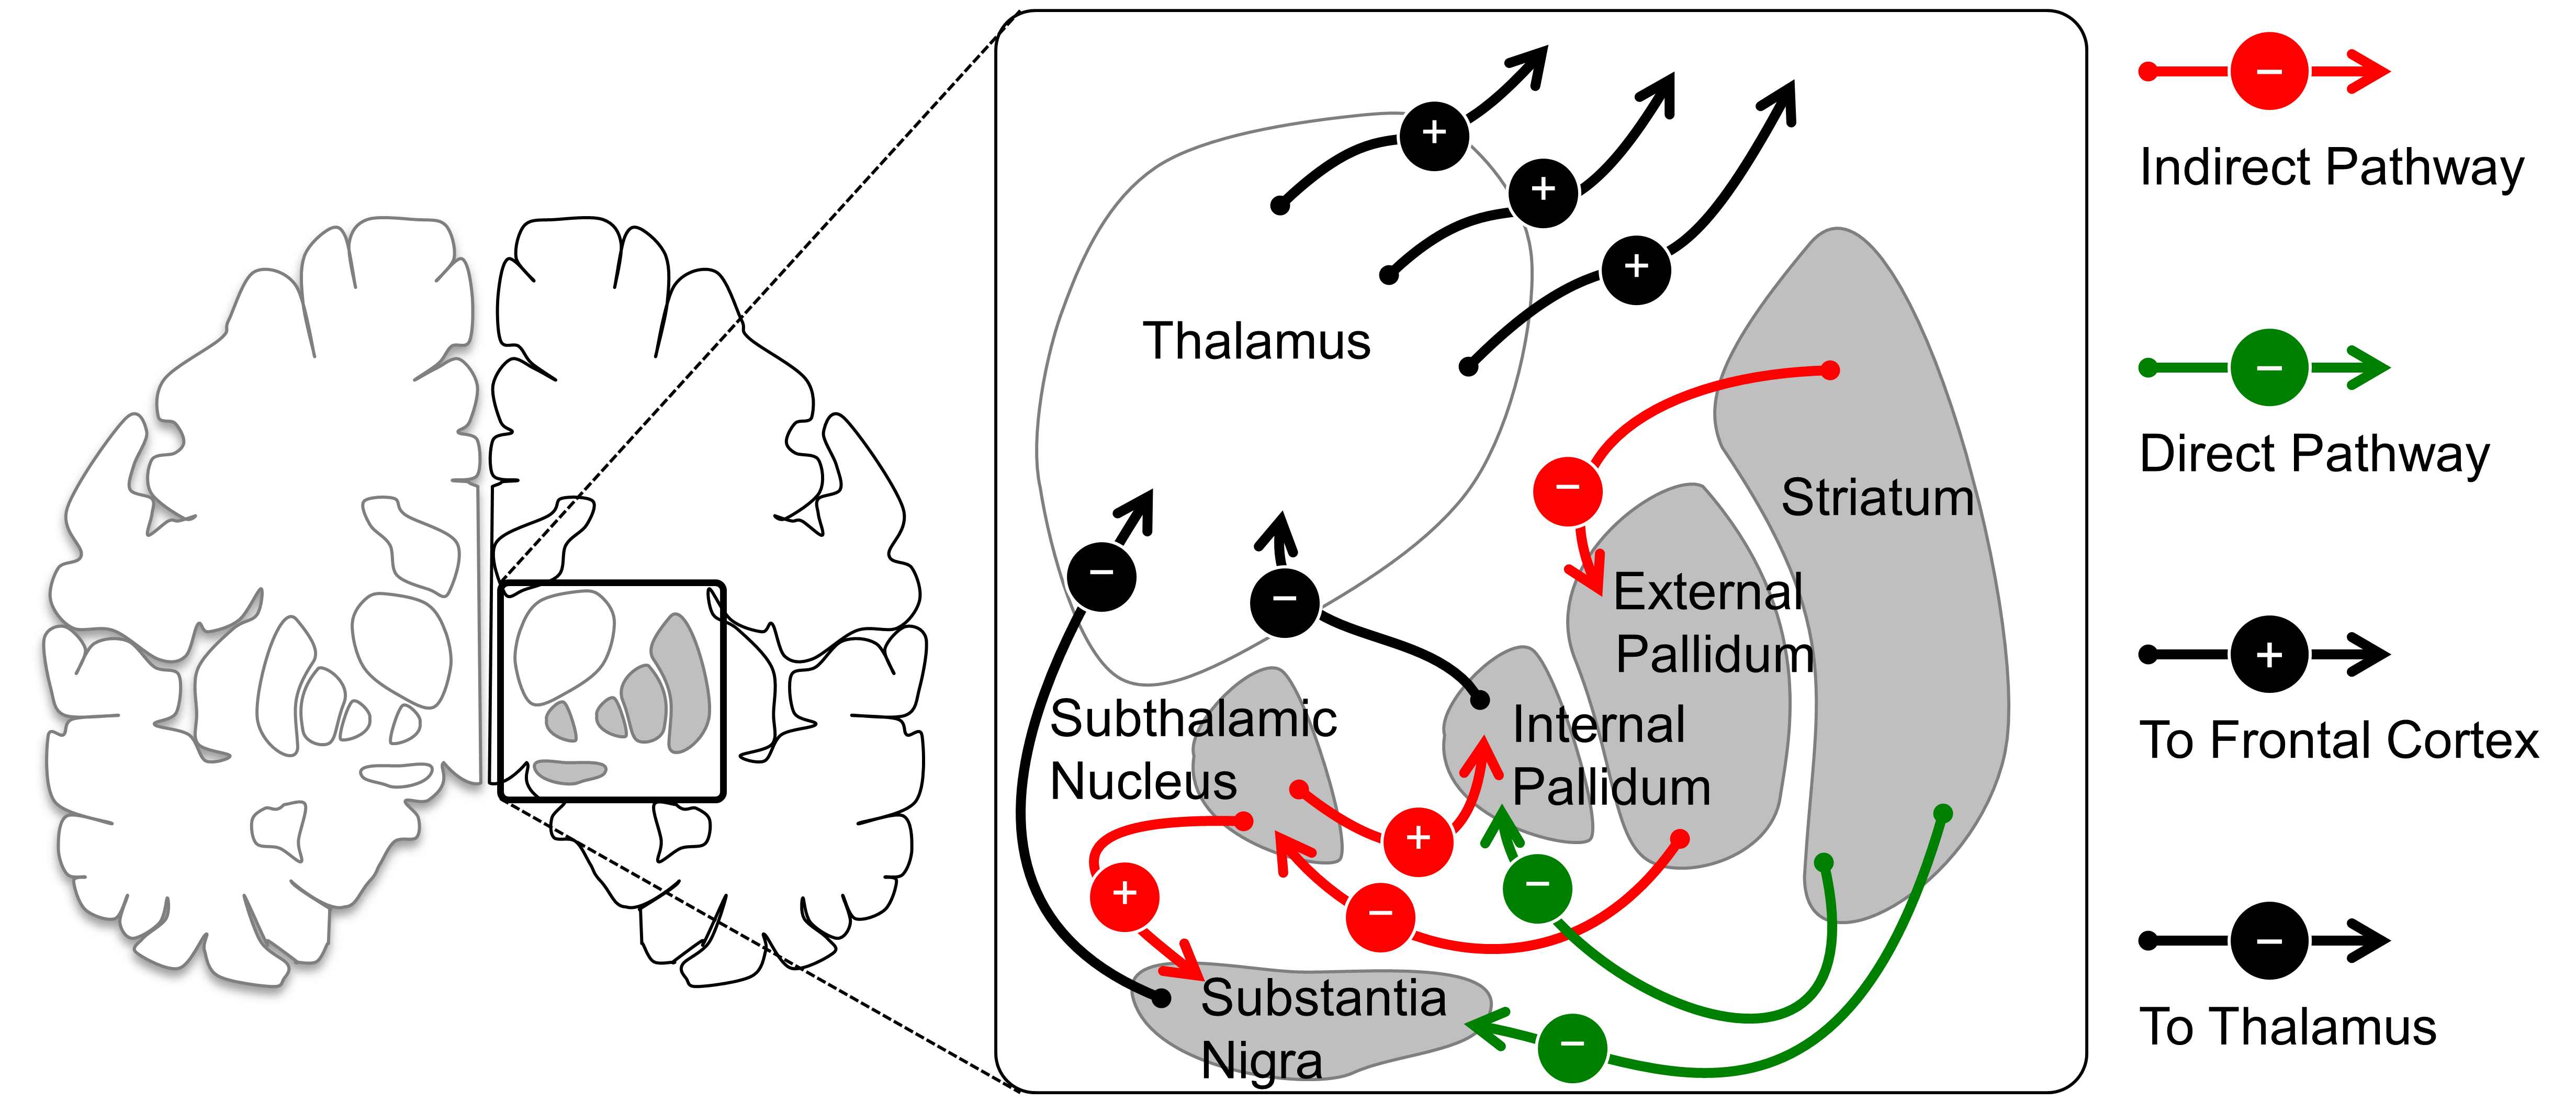
\includegraphics[width=3.5in]{basal-ganglia.png}
	\end{center}
	\caption{The basal ganglia} 
	\label{pss}
\end{figure}

What would a model that does this look like? In order to begin forming an idea, inspiration can be found in natural phenomena that are modeled well, but incompletely, by model-free RL methods. One prevalent example of such is the basal ganglia (BG) system, a network of subcortical nuclei including the striatum, globus pallidus, substania nigra, and subthalamic nucleus (CITE ME!). Along with the cerebral cortex, thalamus, and brainstem, these structures form segregated, parallelized loop circuits (including motor, cognitive, and limbic circuits) in humans and other vertebrates. The striatum receives input from cortical structures, and subsequently propagates the signal to later nuclei of the BG through two distinct pathways, termed the “direct” and “indirect” pathways. ADD SENTENCE OR TWO ABOUT WHAT THESE PATHWAYS ARE SUPPOSED TO DO These loop circuits have been implicated to be involved in eye movements, motivation, decision making, working memory, and most notably, action selection (ANDREA: THE FLESH OF MY FINGERS BURNED AS I WROTE THAT)(CITE ME!). 


	
Of particular interest to neurological/psychological research is the fact that the striatum receives strong dopaminergic (dopamine; DA) input from the substantia nigra pars compacta (SNc). Dopaminergic signaling originating from the SNc has long been thought to reflect a neural “reward” signal associated with internally-generated action and external stimuli (CITE ME! WRITE MORE ABOUT ME?) that the organism has learned is, or expects to be, rewarding in some manner. Additionally, dopaminergic input defines the “direct” and “indirect” pathways mentioned above – striatial neurons that express D1 receptors (for which DA is an excitatory ligand) form the origin of the direct pathway, while those that express D2 receptors (for which DA is an inhibitory ligand) form the origin of the indirect pathway.

Why are RL methods well suited to modeling the basal ganglia? In 1997, Schultz, Dayan, and Montague noted the correspondence of the dopamine signal received by the striatum to the error term utilized by TD learning methods. Rather than signaling the actual magnitude of reward, Schultz et. al. found that midbrain dopamine signals reflected the error between what was expected to be the reward and the actual reward received. When an unexpected reward occurred, dopamine activity phasically increased, time-locked to reward delivery. However, when conditioned to expect reward delivery indicated by some preceding stimulus, this phasic dopamine activity became time-locked to the stimulus presentation while absent from actual reward delivery. Additionally, when expected reward was omitted, a phasic decrease (time-locked to the expectation of when the reward should be delivered) in dopaminergic signaling was observed. 

Since this realization, RL models of many of the BG-ascribed behaviors described above have found success in closely modeling human behavior (CITE ME), and additional RL signals have been identified in the BG, furthering the apparent correspondence between the biological structure and theoretical framework (CITE ME). However, despite this growing evidence of the similarity between BG functioning and RL approaches, the modeling literature has rarely addressed (CITE THE RARE OCCURENCES?) one of the crucial structural features of the basal ganglia – the presence of the distinct direct and indirect pathways. Superficially, there seems to be an obvious compatibility between the necessity for a PSS-task RL model to simultaneously estimate the value both the “chosen” and “not chosen” alternatives within a PSS trial, and DA’s opposing influence on the direct and indirect pathways. Would a model-free RL agent with two “action pathways” perform any better than the “standard” model described above?

In order to implement the two-pathway concept, the Gibbs agent described above was modified to include an opposite set of actions (-A, -B, …, -F), which, when chosen by the agent, result in the selection of the other option that they are paired with. The original set of actions (A, B, …, F) can be conceptualized as the set of actions available to be suggested by the direct pathway (restricted by actions possible within the current state), while the “antiset” can be conceptualized as the set of actions available to be suggested by the indirect pathway (also restricted by the state). So, if the current state (trial) is S = (A,B), and the agent selects the indirect pathway’s action -A, the result is the selection of option B. Figure 3A shows that the simple addition of an “indirect pathway” to the RL model results in a marked absence of the bias observed in the “standard” RL model – as the value of T decreases, both choose and avoid accuracies increase commensurately. As such, the model no longer needs to “trade off” increasing the accuracy for one class of action by becoming less confident in the valuations of the other class of action. Instead, for every choice made, it simultaneously learns both the value of the option chosen, and the value of not choosing the alternative. However, note that the maximum Choose and Avoid accuracies of the BG-plausible model do not quite achieve the same level of accuracy as the “standard” RL models – the uncertainty that the “standard” model had been attributing to the option not chosen has now been distributed across both available options.  Figure 3B demonstrates that overall, the BG-plausible model achieves essentially the same level of global mean accuracy as the “standard” models, without the cost of increasing estimate error. 
	
As described, this implementation of “direct” and “indirect” pathways in the RL model does well at capturing the competition between the direct and indirect pathways of the BG, and alleviates the problem of increasing estimate error with increasing accuracy. However, the BG-plausible model still performs similarly to the “standard” RL models in terms of global mean accuracy, indicating that although the BG-plausible model has improved ability to estimate the value of all options in the environment, this does not translate to improved fitness within the environment. However, just as the “standard” models were missing a crucial aspect of BG physiology (the presence of dual pathways), the BG-plausible model is missing a crucial feature of these dual pathways – the fact that DA signaling has opposite effects on the direct (excitation, mediated through D1 receptors) and indirect (inhibition, mediated through D2 receptors) pathways. 
	
	
To capture the aspect of BG neurodynamics, the BG-plausible RL models was modified so that the learning algorithm results in opposite changes for the actions to the two pathways (an anti-correlated BG-plausible model). Figure 4A shows the results of simulations ran with this model. At minimum values of T, the maximum mean Choose and Avoid accuracies increase slightly, when compared to the original BG-plausible model. Figure 4B shows that similar to the original BG-plausible model, the mean accuracy of the anti-correlated BG-plausible model increases without a subsequent increase in estimate error. Additionally, the small increase in Choose and Avoid accuracies at minimum values of T translate into significantly better overall performance for the anti-correlated BG-plausible model. 
However, what is most striking about the anti-correlated BG-plausible model is that at relatively large values of T (where the action selection process is noisy), the model performs much better than either the original BG-plausible model, or the “standard” RL models. This is an indication that the presence of the anti-correlated pathways in the second BG-plausible model bestow a greater resistance to internal noise than the original BG-plausible model and “standard” RL models possess. Figure 5A more clearly demonstrates this effect: across the range of tested values of T, the mean accuracies of the original BG-plausible model are almost identical to the “standard” RL model (in fact, the “standard” Gibbs RL model performs slightly better at some intermediate values of T). However, across the same range of T values, the anti-correlated BG-plausible model performs much better in almost every circumstance. The model does not perform as well as the “standard”/“original BG” models only when the value of T is very close to zero, indicating almost no noise in the action selection process. A similar analysis can be performed for the model’s estimate error, as seen in Figure 5B. This again shows that for every tested value of T, there is little or no difference between either BG-plausible model – the presence of the two pathways allows each model to accurately estimate the value of both Choose (A, C, and E) and Avoid (B, D, and F) options. However, the “standard” RL model shows significant estimation biases as the lowest levels of noise, when the model’s performance is at a maximum.
	In conclusion, I’m having a really hard time writing this without being very repetitive – I will try tomorrow

Indent the first line of each paragraph by 1/8~inch (except for the
first paragraph of a new section). Do not add extra vertical space
between paragraphs.


\section{First-Level Headings}

First level headings should be in 12~point, initial caps, bold and
centered. Leave one line space above the heading and 1/4~ line space
below the heading.


\subsection{Second-Level Headings}

Second level headings should be 11~point, initial caps, bold, and
flush left. Leave one line space above the heading and 1/4~ line
space below the heading.


\subsubsection{Third-Level Headings}

Third-level headings should be 10~point, initial caps, bold, and flush
left. Leave one line space above the heading, but no space after the
heading.


\section{Formalities, Footnotes, and Floats}

Use standard APA citation format. Citations within the text should
include the author's last name and year. If the authors' names are
included in the sentence, place only the year in parentheses, as in
\citeA{NewellSimon1972a}, but otherwise place the entire reference in
parentheses with the authors and year separated by a comma
\cite{NewellSimon1972a}. List multiple references alphabetically and
separate them by semicolons
\cite{ChalnickBillman1988a,NewellSimon1972a}. Use the
et~al. construction only after listing all the authors to a
publication in an earlier reference and for citations with four or
more authors.


\subsection{Footnotes}

Indicate footnotes with a number\footnote{Sample of the first
  footnote.} in the text. Place the footnotes in 9~point type at the
bottom of the page on which they appear. Precede the footnote with a
horizontal rule.\footnote{Sample of the second footnote.}


\subsection{Tables}

Number tables consecutively; place the table number and title (in
10~point) above the table with one line space above the caption and
one line space below it, as in Table~\ref{sample-table}. You may float
tables to the top or bottom of a column, set wide tables across both
columns.

\begin{table}[!ht]
\begin{center} 
\caption{Sample table title.} 
\label{sample-table} 
\vskip 0.12in
\begin{tabular}{ll} 
\hline
Error type    &  Example \\
\hline
Take smaller        &   63 - 44 = 21 \\
Always borrow~~~~   &   96 - 42 = 34 \\
0 - N = N           &   70 - 47 = 37 \\
0 - N = 0           &   70 - 47 = 30 \\
\hline
\end{tabular} 
\end{center} 
\end{table}


\subsection{Figures}

All artwork must be very dark for purposes of reproduction and should
not be hand drawn. Number figures sequentially, placing the figure
number and caption, in 10~point, after the figure with one line space
above the caption and one line space below it, as in
Figure~\ref{sample-figure}. If necessary, leave extra white space at
the bottom of the page to avoid splitting the figure and figure
caption. You may float figures to the top or bottom of a column, or
set wide figures across both columns.

\begin{figure}[ht]
\begin{center}
\fbox{CoGNiTiVe ScIeNcE}
\end{center}
\caption{This is a figure.} 
\label{sample-figure}
\end{figure}


\section{Acknowledgments}

Place acknowledgments (including funding information) in a section at
the end of the paper.


\section{References Instructions}

Follow the APA Publication Manual for citation format, both within the
text and in the reference list, with the following exceptions: (a) do
not cite the page numbers of any book, including chapters in edited
volumes; (b) use the same format for unpublished references as for
published ones. Alphabetize references by the surnames of the authors,
with single author entries preceding multiple author entries. Order
references by the same authors by the year of publication, with the
earliest first.

Use a first level section heading for the reference list. Use a
hanging indent style, with the first line of the reference flush
against the left margin and subsequent lines indented by 1/8~inch.
Below are example references for a conference paper, book chapter,
journal article, technical report, dissertation, book, and edited
volume, respectively.

\nocite{ChalnickBillman1988a}
\nocite{Feigenbaum1963a}
\nocite{Hill1983a}
\nocite{OhlssonLangley1985a}
\nocite{Lewis1978a}
\nocite{NewellSimon1972a}
\nocite{ShragerLangley1990a}


\bibliographystyle{apacite}

\setlength{\bibleftmargin}{.125in}
\setlength{\bibindent}{-\bibleftmargin}

\bibliography{CogSci_Template}


\end{document}
